\chapter{Annexes}

\section{Planification du projet}
La figure ci-dessous présente le planning de projet, avec un suivi itératif de l'avancée.

\begin{figure}[h]
    \centering
    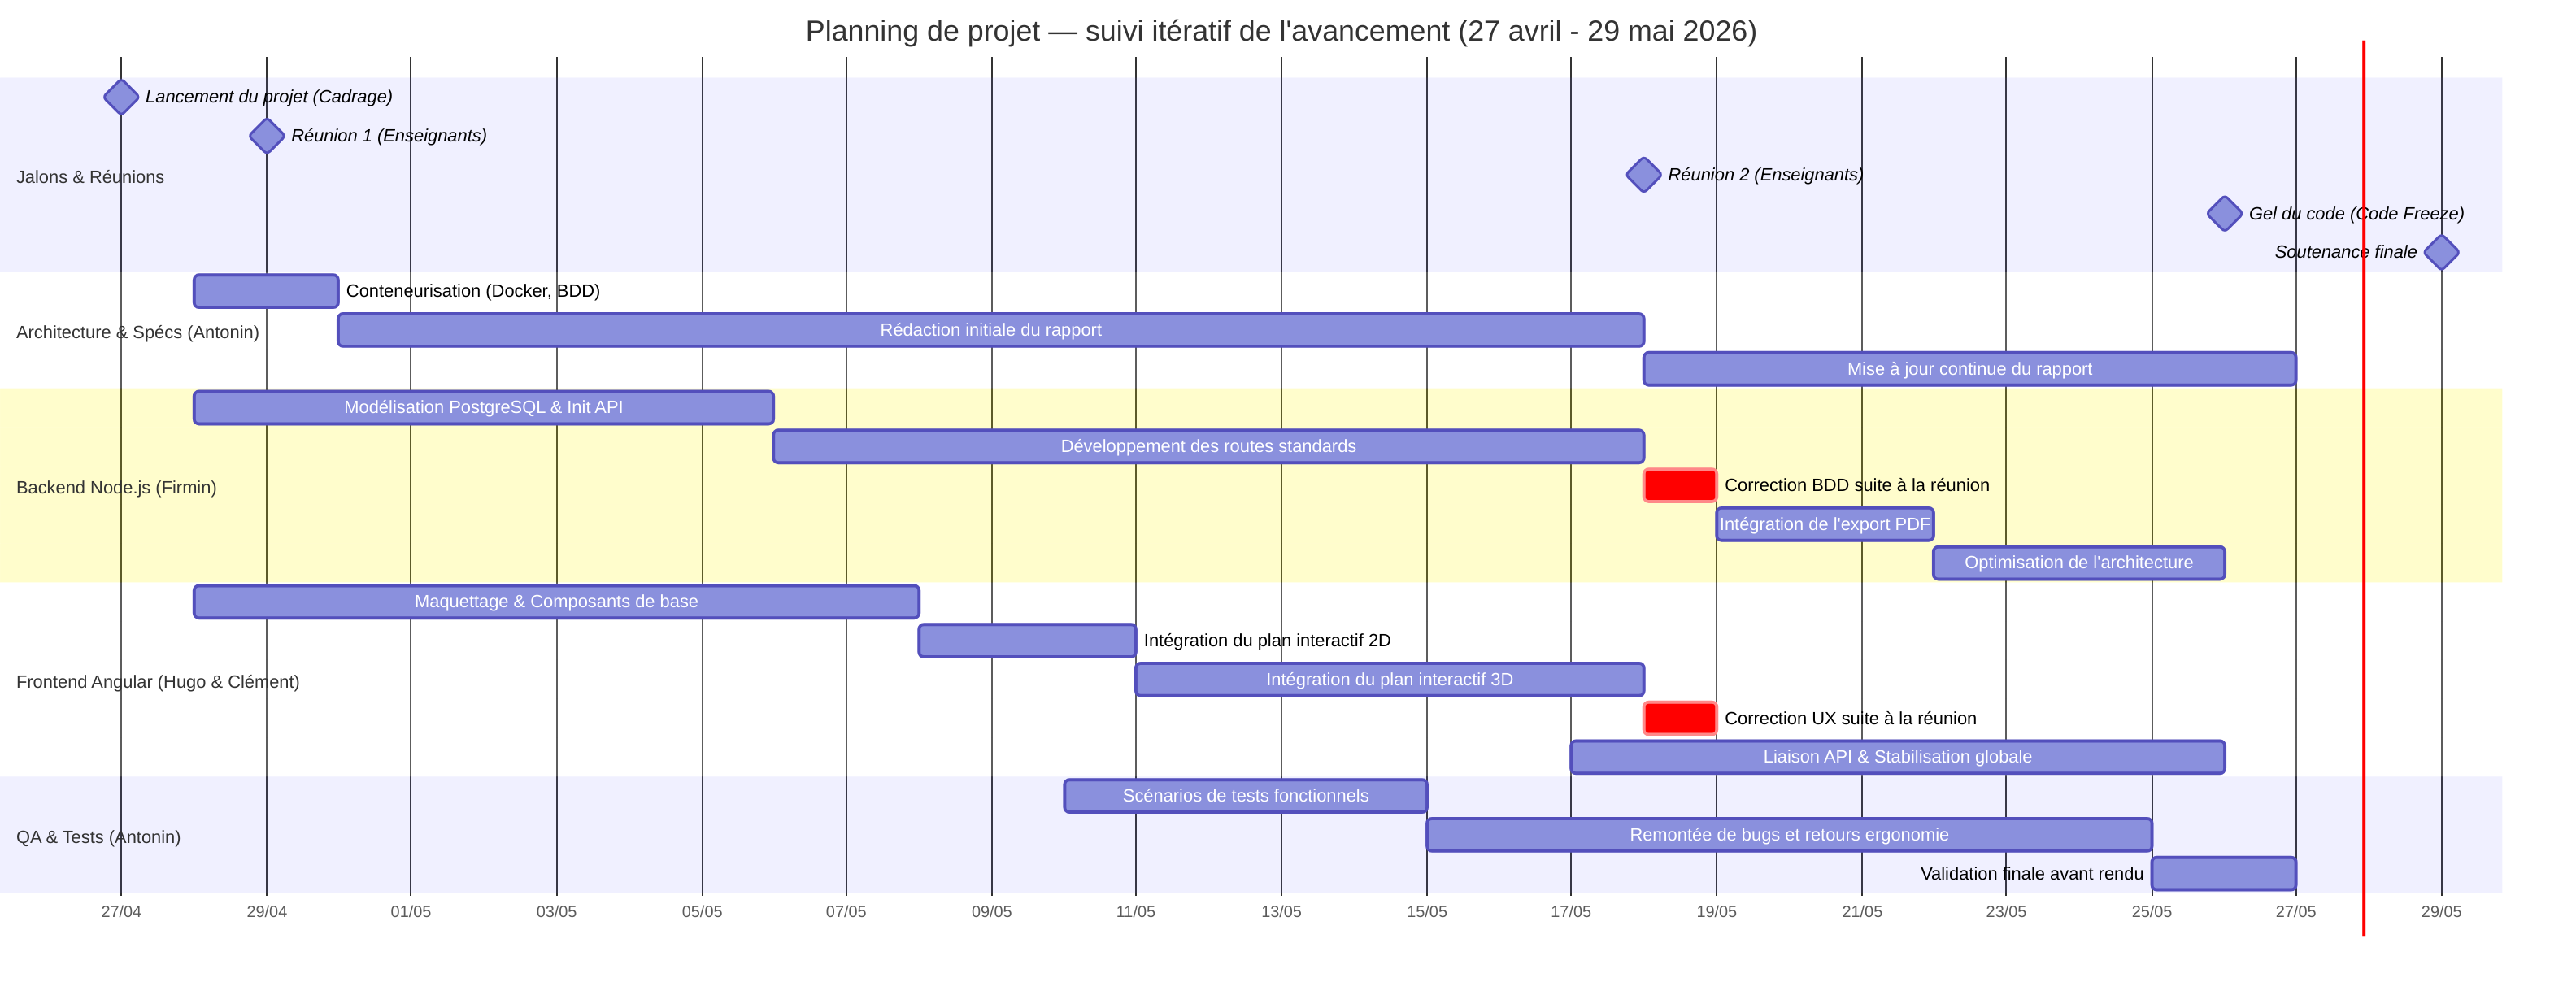
\includegraphics[width=\linewidth,keepaspectratio]{img/diagramme_gantt.png}
    \caption{Planning de projet — suivi itératif de l'avancement}
    \label{fig:gantt}
\end{figure}

\section{Code source et Déploiement}
L'intégralité du code source ainsi que la dernière version packagée de l'application (Release) sont accessibles via le lien ci-dessous. Le téléchargement inclut l'environnement de conteneurisation permettant de lancer l'application immédiatement.

\begin{figure}[h]
    \centering
    \begin{minipage}{0.28\textwidth}
        \centering
        
\includegraphics[width=0.8\linewidth]{img/github_qr.png}
    \end{minipage}\hfill
    \begin{minipage}{0.68\textwidth}
        \centering
        \vspace{1em}
        \href{https://github.com/HugoMagret/Gestion_locaux/releases/latest}{\url{https://github.com/HugoMagret/Gestion_locaux/releases/latest}}
    \end{minipage}
    \caption{Accès direct à la dernière version (Release) du projet}
    \label{fig:github}
\end{figure}

\section{Structure JSON d'un étage} \label{annexe:json_etage}
Le listing ci-dessous présente un extrait du format JSON utilisé pour la définition des plans. Ce format standardisé permet à l'application Angular de générer dynamiquement les vues 2D et 3D, tout en assurant l'intégrité des données lors de l'insertion en base via Node.js.

\begin{verbatim}
{
  "level": 1,
  "rooms": [
    {
      "name": "Salle Réunion",
      "max_capacity": 15,
      "room_type_label": "Réunion",
      "color": "#1abc9c",
      "doors_count": 1,
      "coordinates": { "x": 250, "y": 50, "width": 120, "height": 80 }
    },
    {
      "name": "Bureau 204",
      "max_capacity": 4,
      "room_type_label": "Bureau",
      "color": "#3498db",
      "doors_count": 2,
      "coordinates": { "x": 150, "y": 50, "width": 80, "height": 120 }
    }
  ],
  "doors": [
    {
      "coordinates": { "x": 230, "y": 90, "width": 10, "height": 20 }
    }
  ]
}
\end{verbatim}